\makeatletter\@specialfalse\makeatother

\cxset{
 toc image =,
 name={},
 numbering=arabic,
 number font-size= LARGE,
 number font-family= rmfamily,
 number font-weight= bfseries,
 number before=,
 number dot=,
 number after=\par\offinterlineskip,
 number position=leftname,
 chapter font-family= sffamily,
 chapter font-weight= normalfont,
 chapter font-size= Large,
 chapter before={\vspace*{15pt}\par},
 chapter after=,
 number color=black!90,
 %
 title margin top=30pt,
 title margin bottom=20pt,
 chapter title align=left,
 chapter title text-align=left,
 chapter title width=\textwidth,
%
  title before={},
 title after=,
 title font-family= sffamily,
 title font-color= black,
 title font-weight= bfseries,
 title font-size= LARGE,
 title spaceout=none,
 header style= plain,
 section font-size=Large,
 section color=black,
 section numbering prefix=\thechapter.,
 section indent=0pt,
 }


\chapter{Introduction to Style One}
\addcontentsline{toc}{section}{Template 1 (style01)}
\cxset{headings ruled-01}

\begin{summary}
This design is simple and its distinguishing characteristic is a short summary at the beginning of the chapter. This is almost like an abstract typeset in italic font without setting the margins in. We provide a \lstinline{summary} environment for convenience. Note the very simple line in the running head to the left of the page number.
\end{summary}

\medskip
\begin{figure}[ht]
\centering
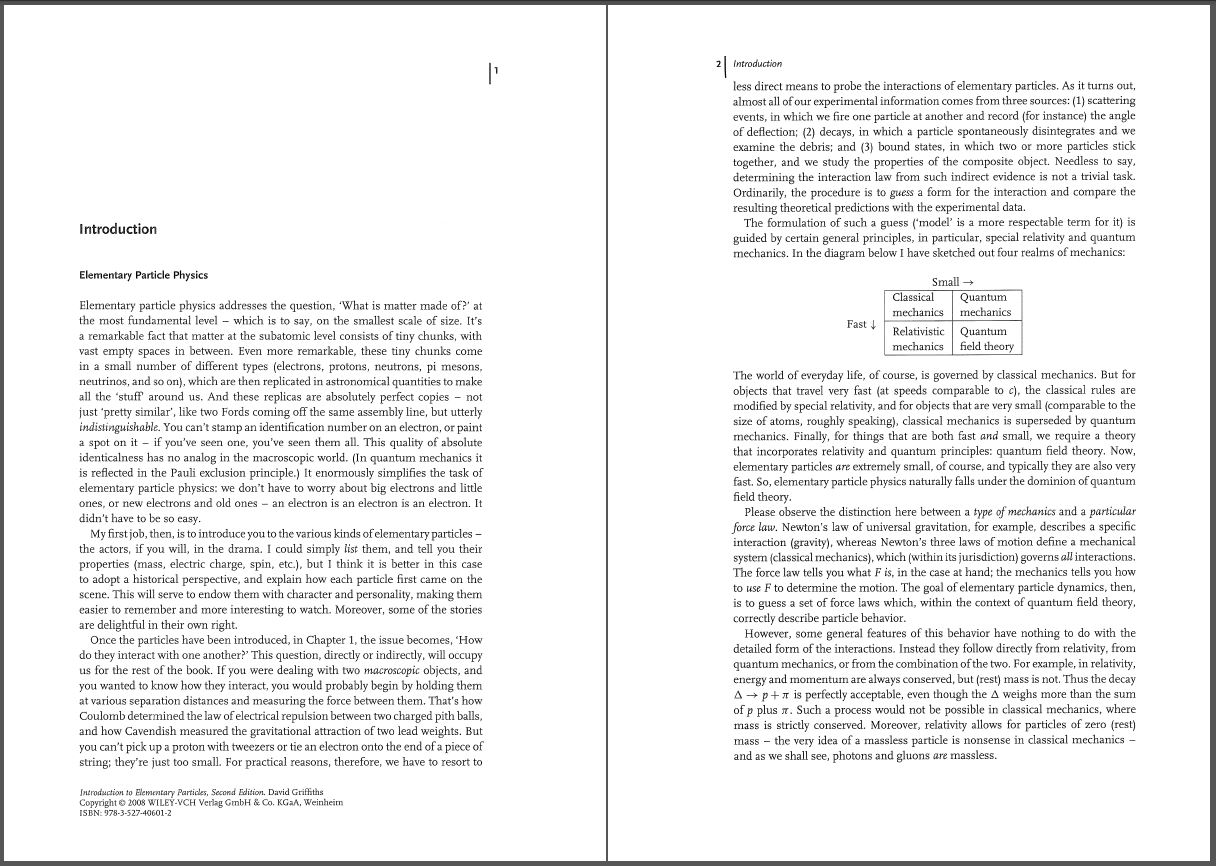
\includegraphics[width=\textwidth]{./chapters/chapter01.jpg}
\end{figure}

The summary after the chapter head can easily be incorporated using \textit{summary}. You
can also use \string\begin\meta{abstract}. The latter will produce a heading with the word, abstract.
Both the summary as well as the abstract can take parameters to be set, for internationalization and to typeset
the words abstract, or summary. If you use \textit{precis}, the summary will be added into the Table of Contents as
well.

I originally picked this style, as a boringly easy style to develop, but it proved a hard nut to crack when it came to sections. Both the section numbering as well as the caption of figures, proved to be difficult to style using
the build-in \latexe commands. 

\section{Images and Figures}

Images and figures are using traditional captions with the exception they are restricted in a certain portion of the textwidth. The word Fig. is abbreviated to Fig. and uses a dot.

\captionsetup[figure]{format = plain,
                                 width=.67\textwidth,
                                 justification=justified,
                                 singlelinecheck=false,
                                 name=Fig.,
                                 labelsep=space,
                                 oneside,
                                 margin=0pt
                                 }

\begin{figure}[ht]
\includegraphics[width=\textwidth]{./images/elementary-images.jpg}
\caption{Note the abbreviation and the restriction of the caption to\\
 a minipage. This combined with the width option manages\\
  the typesetting well.}
\end{figure}

I had to make a special style to capture this. It is unbelievable that a piece of textblock can get so complicated and this particular style, let me to re-think some of the concepts in the phd design. the complication that arises here
is that with most images measuring the image is necessary. The narrower image in the figure would of course not work on the same settings, and the caption is at the full width of the figure, as shown below.













\makeatother
